\documentclass[addpoints]{exam}

\usepackage{graphbox}
\usepackage{hyperref
}\usepackage{subcaption}
\usepackage{titling}

% Header and footer.
\pagestyle{headandfoot}
\runningheadrule
\runningfootrule
\runningheader{CS 201}{Homework 4}{\theauthor}
\runningfooter{}{Page \thepage\ of \numpages}{}
\firstpageheader{}{}{}

\qformat{{\large\bf \thequestion. \thequestiontitle}\hfill[\totalpoints\ points]}
% \qformat{{\large\bf \thequestion. \thequestiontitle}\hfill}
\boxedpoints

\noprintanswers

\graphicspath{{images/}}

\title{Homework 4: Art in the Structures }
\author{CS 201 Data Structures 2\\
By Ayeza Nasir , Fatima Alvi , Sudais Yasin }
\date{Spring 2022}

\begin{document}
\maketitle

\section*{Introduction}
This Homework had us quite confused as to how to best elaborate on and express our semesters findings in this course through art , We took to researching and ideating over the course of the weekend to come up with a few pieces that we are happy with and we hope you enjoy looking at them too. 

\section*{Abstract Image I}

\begin{figure}[h]
\footnotesize  
  
    
        \begin{center}
              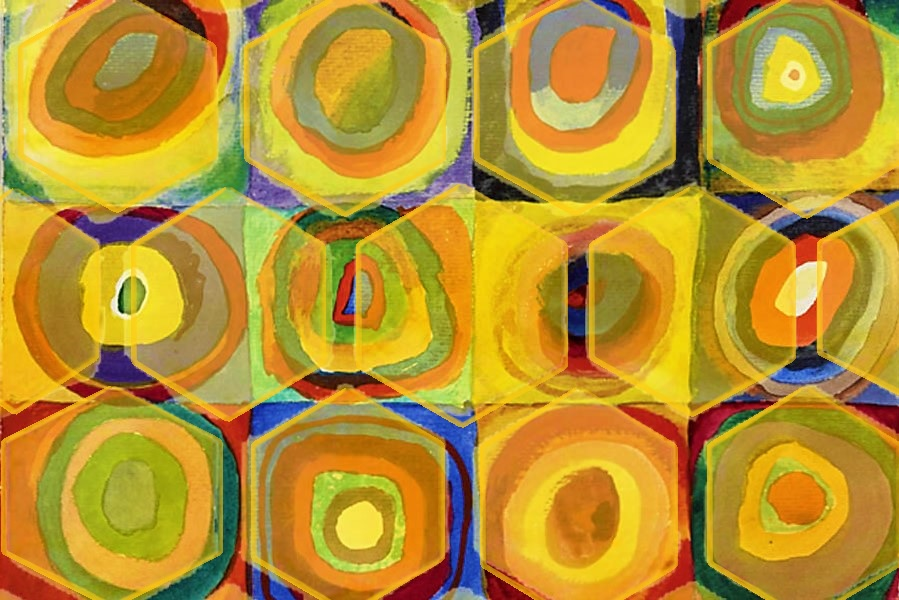
\includegraphics[height=.3\textheight, align=c]{myimage1}
        \end{center}
  

  \caption{Wassily Kadinsky's Language of Color embossed with a honey comb Structure} 
  \label{fig:example}
\end{figure}

\section*{Accompaniment}

 When we were searching for ideas for how to artistically explain and express our journey within the ream of the Data Structures II course , we came across numerous ideas , where as this painting by \textbf{Wassily Kadinsky} a very famous Russian painter stood out to us the most , it is a painting a circles contained in boxes with layers and layers of different colors, As we know circle is the least restrictive shape which we find to be artistically very elaborate ,In Figure \ref{fig:example} ,  We saw these boxes as individual frameworks and the circles contained within them  as a data structure each , We can see some circles have similar layering of color , as we have learned in this course that some data structures also share similar properties and purposes , a great example of these would be the family of Trees data structures , B- Trees , Red- Black Trees , Binary Search trees and numerous more , do seem to share a set of certain similar features but are entirely different entities in their implementation . We embossed this image with a hive pattern drawn via paint which was inspired inspired by honey combs because honey combs are symbolic are symbolic of space utilisation and optimization, the hexagonal structuring in a bee hive , utilises the same amount of space whilst using less material , which is reflective of the structures we have come across in this course. Space and complexity are two of the most major concerns in data structures hence to encapsulate this idea we decided to use these 2 images to digitally create a abstract expression to capture features such as order, structure, organization, ingenuity of our learning and journey in the DS2 course. 

\section*{Abstract Image II}

\begin{figure}[h]
\footnotesize  
  
    
        \begin{center}
              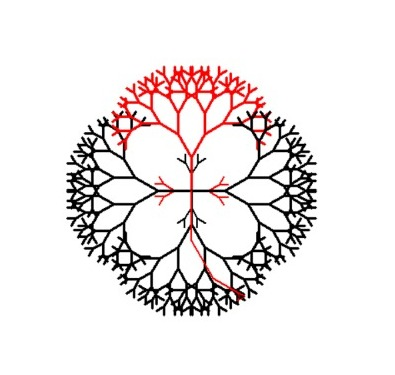
\includegraphics[height=.2\textheight, align=c]{tree1}
        \end{center}
          \begin{center}
              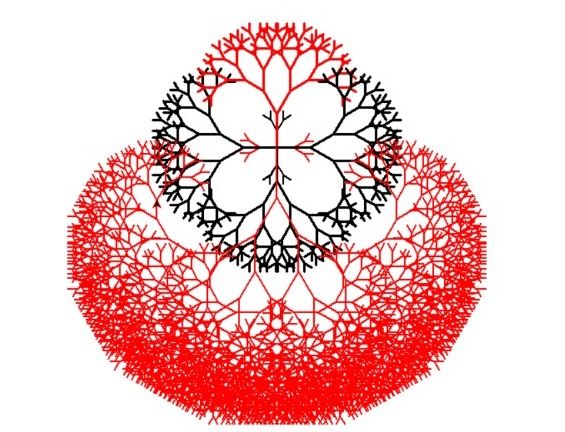
\includegraphics[height=.2\textheight, align=c]{tree2}
        \end{center}
           \begin{center}
              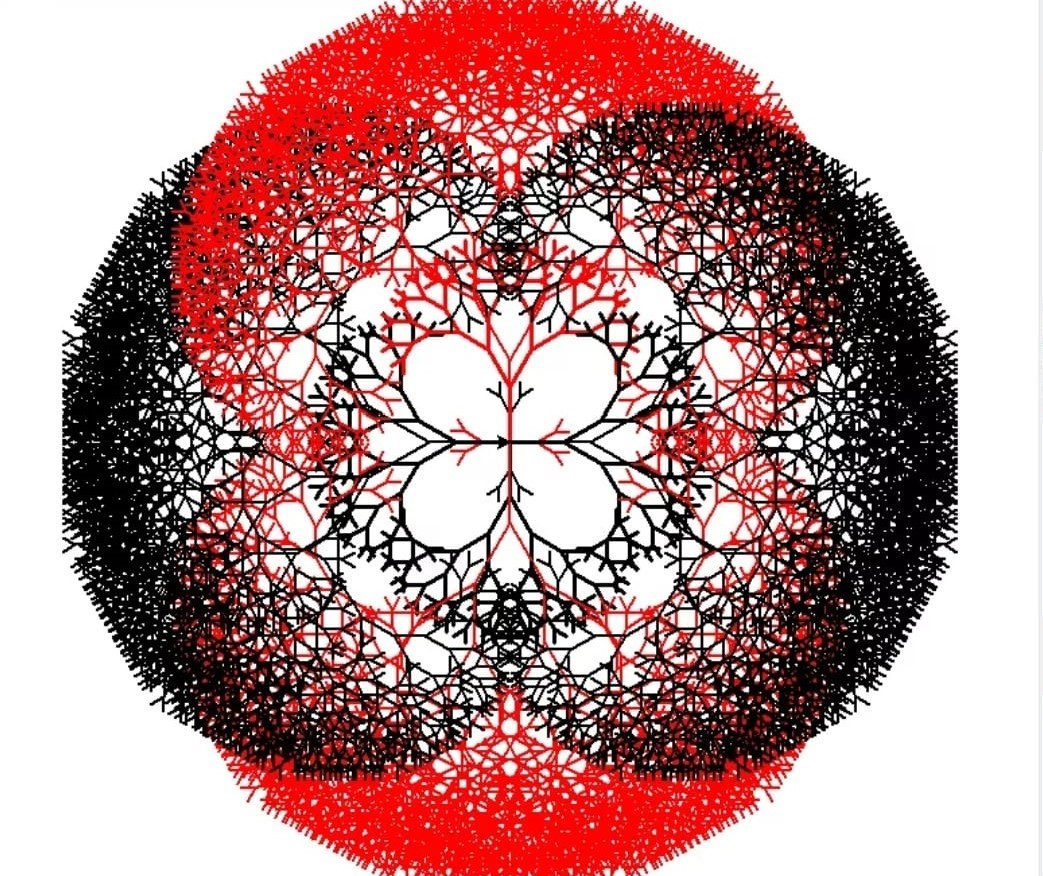
\includegraphics[height=.2\textheight, align=c]{tree3}
        \end{center}
  
  \caption{Abstract Art Pattern Implemented in Python3 Via Fractal Trees} 
  
\end{figure}

\section*{Accompaniment II }

This is a programmed  Pythagorean tree, intended to reflect on the red-black tree in an artistic way which we learned about in this course. It isn't just red and dark, yet it is moreover, in a real sense, reflects the branching, root structure, and shape of a real-life tree too! We can see the astonishing properties of balance in tree by the symmetry we observed in this tree too. From root presumed to be the centre to the leaf the growth of the tree is similar corresponding to the real implementation of Red-Black trees
This tree likewise follows red-black tree properties  \\
1)It starts with a black node.\\
2)Every branch end can be interpreted as  leaf which  is a special node called NIL (with no key).\\
3) No Red node can have black child .

The code was composed in python and inspired by the book Chaos and, Fractals'.




\section*{References}
\begin{center}

\begin{enumerate}
    \item https://www.csmonitor.com/The-Culture/The-Home-Forum/2013/0411/Kandinsky-spoke-language-of-color
    \item https://www.educative.io/edpresso/what-is-a-red-black-tree
\end{enumerate}
\end{center}

\bigskip

\hrulefill \textit{Hope you enjoyed!} \hrulefill

\end{document}

%%% Local Variables:
%%% mode: latex
%%% TeX-master: t
%%% End: